\documentclass[conference]{IEEEtran}
\usepackage{blindtext, graphicx}
\usepackage{amsmath}
\usepackage{listings}
\usepackage{booktabs}
\usepackage{multirow}
\usepackage{tabularx}

\ifCLASSINFOpdf
\else
\fi


% correct bad hyphenation here
\hyphenation{op-tical net-works semi-conduc-tor}


\begin{document}

% figures: only your own research
% paraphrases
% clearer statements related to the findings

\title{Redesigning CHIML: Orchestration Language for Chimera-Framework}

\author{\IEEEauthorblockN{Go Frendi Gunawan}
\IEEEauthorblockA{STIKI Malang\\ Malang, Indonesia\\
Email: frendi@stiki.ac.id}
\and
\IEEEauthorblockN{Jozua Ferjanus Palandi}
\IEEEauthorblockA{STIKI Malang\\
Malang, Indonesia\\
Email: jozuafp@stiki.ac.id}
\and
\IEEEauthorblockN{Subari}
\IEEEauthorblockA{STIKI Malang\\
Malang, Indonesia\\
Email: subari@stiki.ac.id}}


% make the title area
\maketitle


\begin{abstract}
%\boldmath
Component Based Software Engineering (CBSE) has been proven to be quite effective to deal with software complexity. Nowadays developers prefer to build micro-services rather than single monolithic application. Several SOA (Service Oriented Architecture) approaches like HTTP/REST API, CORBA, and BPEL are commonly used by developers. Some of those solutions are built under assumptions that the developers are either building the services from scratch or able to create abstraction layer for the pre-existing services. In most cases the assumptions are true. However there are cases when developers prefer to keep the architecture as simple as possible without any need to build additional abstraction layers. For example, when they work with mini-embeded system.

Previously, a YAML based orchestration language was developed for Chimera-Framework (A language agnostic framework for stand-alone and distributed computing). In this paper, we refine the orchestration language in order to let developers accessing pre-existing services without any need to build another abstraction layer.
\end{abstract}

% Note that keywords are not normally used for peerreview papers.
\begin{IEEEkeywords}
Chimera, CBSE, Orchestration Language
\end{IEEEkeywords}

\IEEEpeerreviewmaketitle

\section{Introduction}

Software development is a very interesting topic. The way people developing softwares is changing as new paradigms emerged. In turns, software development also affecting the culture. It change how people interact to each others as well as how they interact with computers.

As software become more and more complex, building and maintaining softwares is also become harder. Various approaches have been attempted in order to make the processes easier.

Several frameworks like Rails, Django, Laravel, etc are focusing on how to make codes clean, separated, and reusable. In turn, this make software development and maintenance easier. These frameworks quickly gained popularity among software developers.

However, despite on the clear advantage of those frameworks, they also have several disadvantages. Since the frameworks were built on top of specific programming language, integration to different programming languages is quite challenging. For example, in order to build software by using Rails, developers should code in Ruby. The same is also true for Django, which is built on top of Python, and Laravel which is built on top of PHP. This situation is known as vendor-lock-in. And in some cases it can affect maintainability as well as further development in a bad way.

Thus, a more technology agnostic approach is needed in order to overcome vendor-lock-in problem. Recently, SOA and micro-services are gaining popularity. Those approaches let developers to focus on small components known as services rather than complex monolithic software. A service usually represent single resource or business process. The services can be independent to each other or aware to each others. Despite of the advantages and popularity, SOA and micro-services are prone to concurrency problem.

One important aspect in SOA/micro-services is how a developer can compose independent services to work together. There are two common approach to compose services. The process to compose several services that are independent to each others is named orchestration, while the process to compose several services that aware to each others is named choreography. Orchestration require one central controller in order to manage the services.

Orchestration has a very long history. The earliest implementation of orchestration was Unix Pipe mechanism. This mechanism is still relevant and used by Unix/Linux users.

Unix Pipe mechanism is not the only implementation of software orchestration. Remote Procedure Call (RPC) is also used for bigger projects. Beside Unix Pipe and RPC Several other implementations were introduced by independent companies and consortiums. OMG introduced CORBA on 1991, while OASIS intoduced BPEL on 2001. Some developers also implement their own HTTP/REST API implementation. On 2016, Feilhauer and Sobotka creating a framework named DEF which is focusing on parallel execution. On 2017, we also conduct a research to develop another language agnostic framework named Chimera-Framework. Recently Google also introduce GRPC.

Compared to the monolithic frameworks like Rails and Django, these orchestration mechanism are more scalable and technology agnostic. This mean that the developers can choose the best technology stack to build their components/services.

Among those orchestration mechanisms, Unix pipe and Chimera-Framework are the only ones that are agnostic to the architecture and messaging protocol. To implement CORBA or BPEL, the developers has to specify IDL or WSDL. In DEF, the similar mechanism named DEF-WS also has to be created. These specifications also assuming that components are HTTP aware. Consequently, the developers need to consider this behavior before creating a new service/component. It doesn't mean that pre-existing components cannot be used for orchestration. However the components are either need refactoring or additional broker. This make the deployment process more complex.

Chimera-Framework in the other hand focusing on how to make the effort minimal. The orchestration components in Chimera-Framework don't have to be HTTP aware. Even an old UNIX utility like `date` or `cat` will serve well.

In this research we are focusing in improving the orchestration mechanism in Chimera-Framework. The orchestration language is named CHIML (Chimera Markup Language) which is a superset of YAML. CHIML is designed to be readable, compact, and intuitive.


\section{Research Question}

In order to have a clear direction in our research, we are focusing in these two questions:

\begin{itemize}
    \item How to make a readable, compact, and intuitive orchestration language for Chimera-Framework.
    \item How the orchestration language compared to other possible solutions.
\end{itemize}

\section{Literature Survey}

\subsection{Orchestration and Choreography}

\subsection{SOA and Micro-service}

\subsection{HTTP/REST API}

\subsection{SOAP}

\subsection{CORBA, BPEL, and EJB}

\section{CHIML}

\subsection{Design}

{\lt CHIML} is a superset of `YAML`. So, any valid `YAML` is also a valid `CHIML`. And as `YAML` itself is a superset of `JSON`, any valid `JSON` is also a valid `CHIML`

\subsection{Semantic (Backus Naur Form)}

\begin{lstlisting}[caption=CHIML Semantic, label=chimlSemantic, basicstyle=\footnotesize, breaklines=true]
<program> ::= 
 <completeVars>
 <completeVerbose>
 <command>
 <completeCatch>
 <completeThrow>

<command> ::=
 | <completeCommand>
 | <shortCommand>

<completeCommand> ::= 
 | <completeIns>
   <completeOut>
   <completeIf>
   "do: "<process><newLine>
   <completeWhile>

 | <completeIns>
   <completeOut>
   <completeIf>
   "parallel: "<process><newLine>
   <completeWhile>

 | <completeIns>
   <completeOut>
   <completeIf>
   "do: "<commandList>
   <completeWhile>

 | <completeIns>
   <completeOut>
   <completeIf>
   "parallel: "<commandList>
   <completeWhile>

 | "map: "<variableName>
   "into: "<variableName>
   <completeCommand>

 | "filter: "<variableName>
   "into: "<variableName>
   <completeCommand>

<shortCommand> ::= 
 | "|("<ins>") -> " <process> " -> " <out><newLine>
 | "|("<ins>") -> " <process> "<newLine>
 | "|"<process> " -> " <out><newLine>
 | "|("<ins>") --> " <out><newLine>
 | "|"<out> " <-- ("<ins>")"<newLine>

<commandList> ::= 
 | "- "<command>
 | <commandList><commandList>

<completeCatch> ::= 
 | "" 
 | "catch: "<condition><newLine>

<completeThrow> ::=
 | ""
 | "throw: "<string><newLine>

<completeVars> ::=
 | ""
 | "vars: "<variableList><newLine>

<completeVerbose> ::=
 | ""
 | "verbose: "<verbosity><newLine>

<completeIns> ::=
 | ""
 | "ins: "<ins><newLine>

<completeOut> ::= 
 | ""
 | "out: "<out><newLine>

<completeIf> ::= 
 | ""
 | "if: "<condition><newLine>

<completeWhile> ::=
 | ""
 | "While: "<condition><newLine>

<ins> ::= <variableList>

<out> ::= <variableName>

<process> ::= 
 | <cliCommand>
 | <jsArrowFunction>
 | "{"<jsNormalFunction>"}"
 | "["<jsFunctionWithCallback>"]"
 | "<"<jsPromise>">"

<variableList> ::= 
 | <variableName>
 | <variableName>","<variableList>

\end{lstlisting}

\subsection{Default Variables}

\subsection{Implementation}

\section{Experiment}

\subsection{Solutions}

\section{Result and Discussion}

\begin{table}[]
\centering
\caption{Simplicity Comparison}
\label{tbl:simplicityTest}
\begin{tabular}{@{}rrrrrrrrr@{}}
\toprule
  b\_real & b\_sys  & b\_user &   fkgl &     fre &  loc & problem  & size &  solution \\
          &         &         &        &         &      &          &      &           \\ \midrule 
  0.246   & 0.022   & 0.236   &  8.390 &  42.035 &  30  &   gba    & 978  &     js    \\
  0.113   & 0.010   & 0.098   & 18.128 & -28.851 &  15  &   gba    & 662  &     py    \\
  0.317   & 0.025   & 0.304   &  7.103 &  50.217 &  17  &   gba    & 554  &  chiml    \\
  0.230   & 0.018   & 0.226   & 11.044 &  22.670 &  16  &    gb    & 540  &     js    \\
  0.101   & 0.013   & 0.087   & 15.674 & -11.228 &  12  &    gb    & 471  &     py    \\
  0.310   & 0.026   & 0.294   &  4.516 &  68.987 &  13  &    gb    & 381  &  chiml    \\
  0.221   & 0.021   & 0.214   & 19.039 & -35.587 &   7  &     g    & 250  &     js    \\
  0.095   & 0.010   & 0.084   & 17.319 & -23.463 &   6  &     g    & 217  &     py    \\
  0.293   & 0.020   & 0.287   &  4.613 &  68.522 &   6  &     g    & 163  &  chiml    \\
          &         &         &        &         &      &          &      &           \\ \midrule 
\end{tabular}
\end{table}


\begin{figure}
	\centering
	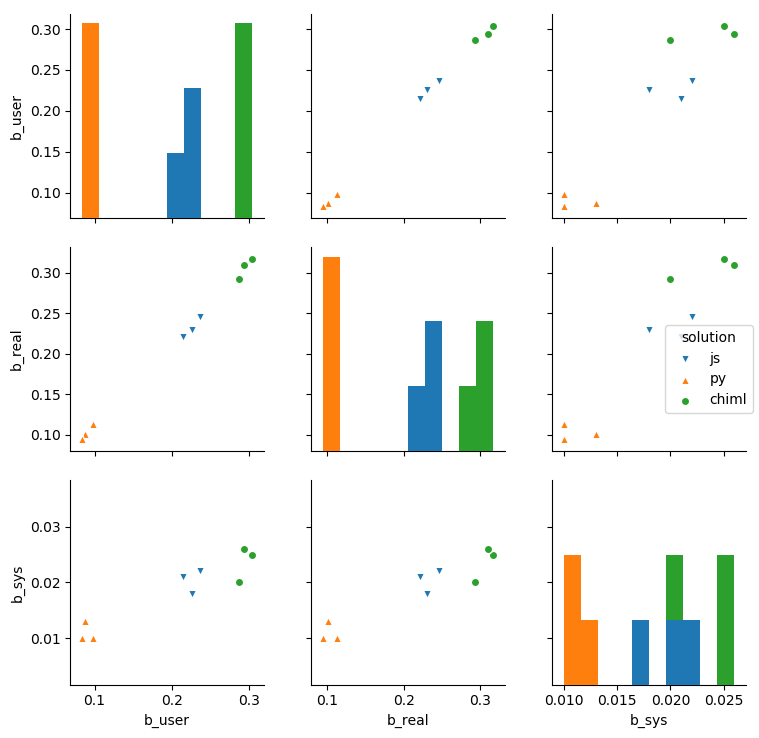
\includegraphics[width=0.3\textwidth]
		{benchmark/benchmark.png}
	\caption{Performance Comparison}
	\label{fig:performanceComparison}
\end{figure}


\begin{figure}
	\centering
	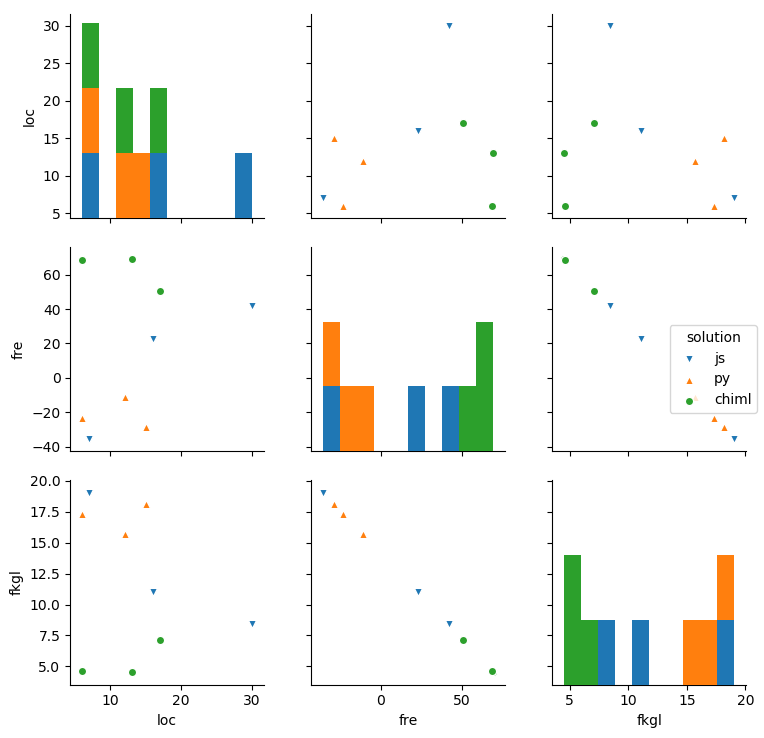
\includegraphics[width=0.3\textwidth]
		{benchmark/readability.png}
	\caption{Readability Comparison}
	\label{fig:readabilityComparison}
\end{figure}

\section{Conclusion}

CHIML serve well as orchestration language. However for control structure, the existance of intermediary components can help to boost performance. The best trait of CHIML is it's support for programming-in-large and programming-in-small. Eventough the control structure is still suffering for speed and performance, it serves well as prototyping tool. This mean that the developer can start orchestration solution in CHIML, then gradually do optimization.

%\appendices
%\section{Proof of the First Zonklar Equation}

% use section* for acknowledgement
%\section*{Acknowledgment}

%The authors would like to thank Sonny Setiawan, Satriyo Wibowo, Dani Devito, and Zusana Pudyastuti for their suggestions and inputs.

% Can use something like this to put references on a page
% by themselves when using endfloat and the captionsoff option.
\ifCLASSOPTIONcaptionsoff
  \newpage
\fi

\bibliographystyle{IEEEtran}
\bibliography{./citation}

% that's all folks
\end{document}

